\section{The Machine Learning Module [Klaus]}

The machine learning part of insieme is mainly designed to pick the best configuration out of several ones. For example it is used to predict the correct splitting of an OpenCL kenerl over all available devices. It is implemented based on the Shark library~\cite{shark}, providing an interface for Artificial Feed Forward Neural Networks (FFNets) and Support Vector Machines (SVMs). \\

During training as well as the classification is based, the features are read/written form/to a database with a certain layout, described in section~\ref{sec:Compiler.Frontend.ml.databaseLayout}. The current implementation uses the Kompex library~\cite{kompex} to access SQLite databases~\cite{sqlite}. \\

The machine learning can either be used by including the corresponding headers in a C++ program or by just using the provided executables. The following code shows an example how to use machine learning in a simple program. \\

\begin{insCode}
#include "ReClaM/Svm.h"
#include "ReClaM/MeanSquaredError.h"
#include "insieme/machine_learning/myModel.h"
#include "insieme/machine_learning/trainer.h"


int main() {
	// set up some parameters
	std::string dbPath = /*path to database file*/;
	size_t nClasses = /*number of classes for the current problem*/;
	
	// construct a SVM
	RBFKernel kernel;
	insieme::ml::MyMultiClassSVM svm(kernel, nClasses); 
	SVM_Optimizer optimizer;
	MeanSquaredError err;
	insieme::ml::Trainer trainer(dbPath, svm, GenNNoutput::ML_KEEP_INT);
	
	// set static/dynamic features to train 
	trainer.setStaticFeaturesByName(/*std::vector containing the names of the desired static features*/);
	trainer.setDynamicFeaturesByName(/*std::vector containing the names of the desired dynamic features*/);
	// set the name of target to train for
	trainer->setTargetByName(/*string with the name of the target*/);
	
	// do the training
	double error = trainer->train(optimizer, err, 0);
	
	// evaluate the trained model using some certain pattern
	Array<double> testPattern;
	/* fill pattern with values to test */
	size_t predictedClass = trainer.evaluate(testPattern);
}
\end{insCode}

This code snipped trains a SVM, for FFNets it work similar, just the shape of the network has to be set up passing a connection matrix of type \type{Array<int>} created with the Shark-provided function \decl{void createConnectionMatrix(Array<int> \&con, Array<unsigned> \&layers, bool ff\_layer, bool ff\_in\_out, bool ff\_all, bool bias)} to the FFnet's constructor. The difference between static and dynamic features is described in Section~\ref{sec:Compiler.Frontend.ml.databaseLayout}. The third argument of \decl{insieme::ml::Trainer(const std::string\& myDbPath, MyModel\& myModel, enum GenNNoutput genOutput = ML\_MAP\_TO\_N\_CLASSES, std::ostream\& outstream = std::cout)} describes how the values of the target in the database are mapped to the different classes. Table~\ref{tab:Compiler.Frontend.ml.GenNNoutput} shows the awailable options. The provided executables listed in Talble~\ref{tab:Compiler.Frontend.ml.execs} always use the option \constant{ML\_KEEP\_INT} since this is the only option currently in use;

\begin{centering}
\begin{threeparttable}[1h]
	\begin{tabular}{l|l}
		\textbf{Flag} & \textbf{Functionality} \\
		\hline \hline
		\constant{ML\_KEEP\_INT}           & Uses the value of the target directly as calss index. \\
		                                   & Floating point values are rounded down. \\
		\constant{ML\_MAP\_FLOAT\_LIN}     & Maps the values to the class indices on a linar scale.\\
		\constant{ML\_MAP\_FLOAT\_LOG}     & Maps the values to the class indices on a lograithmic \\
		                                   & scale. \\
		\constant{ML\_MAP\_FLOAT\_HYBRID}  & Maps the values to the class indices using the \\
		                                   & arithmetic mean of a linear and logarithmic scale. \\
		\constant{ML\_MAP\_TO\_N\_CLASSES} & Sorts all patterns according to their value and divides \\
		                                   & them into classes so that every class has the same \\
		                                   & number of elements. \\
		\hline 
	%	\multicolumn{2}{c}{} \\
	\end{tabular}
	\caption{Flags to be passed to a \type{insieme::ml::Trainer} constructor}
	\label{tab:Compiler.Frontend.ml.GenNNoutput}
\end{threeparttable}
\end{centering}

Talble~\ref{tab:Compiler.Frontend.ml.execs} lists the executables provided within Insieme and their functionality. To see the arguments that the executables accept run it with option '-h'\\

\begin{centering}
\begin{threeparttable}[1h]
	\begin{tabular}{l|l}
		\textbf{Executable} & \textbf{Functionality} \\
		\hline \hline
		\file{train\_ffnet}    & Trains a FFNet based on the options passed to it. The features of\\
		                       & the trainin patterns are read form the passed database. It will train \\
		                       & on all patterns which contain values for all the specified features.  \\ 
		\file{train\_svm}      & Trains a SVM. Except for some SVM/FFNet specific options, the \\
		                       & functionality is equivalent to the one of \file{train\_ffnet}. \\
		\file{evaluate\_model} & Takes a model and a database as a input and evaluates the\\
		                       & classification on the specified patterns \\
		\file{calculate\_pcs}  & Performs principle component analysis and stores the calculated\\
		                       & principle components int he database. \\
		
		\hline
		\multicolumn{2}{c}{} \\
	\end{tabular}
	\caption{Executables generated by the Machine Learning part of Insieme}
	\label{tab:Compiler.Frontend.ml.execs}
\end{threeparttable}
\end{centering}

\subsection{Database Layout}
\label{sec:Compiler.Frontend.ml.databaseLayout}

As mentioned in the previous paragraph, any machine learning action, training and evaluating, is performed based on features which are read from a database. Basically, the \type{insieme::ml::Trainer} and \type{insieme::ml::Evaluator} can deal with any database, since the user can pass any SQL query to them. This query must result in one line for each patten, containing all features (and the target value when doing the training). However, both classes can construct a standard query for a generic number of features. Obviously, this query can only work with a certain database layout, which is illustrated in Figure~\ref{fig:Compiler.Frontend.ml.dbLayout}. In this layout, one can clearly see the strict distinction between static (per code) and dynamic (per setup) features. Also PCA features are handled separately. This structuring arises from the usecase it is designed for: Typically, for one program we have several measurements using different settings. Also the various settings are often the same for all codes. Therefore we choose this layout, in order to minimize the redundancy in the database. The name of static features and their unique id is registered in table \type{static\_fatures}. In the table \type{code} one can find one of these ids in each line, along with the id of a code and the value of this feature for this code. This structure is anolog for the dynamic and PCA features. To generate a query that works on a database with this layout, one has only to specify the desired static and dynamic or PCA features. Note that in the tables for the PCA features only features are written, which consist of a combination of static and dynamic features. If they contain only one kind, they are added to the corresponding static/dynamic tables. Furthermore, the metric to train for (the desired/measured values of the training data set) must be specified. These values are one column int the \type{measurement} table. A database can have many columns of different values to train for. In Figure~\ref{fig:Compiler.Frontend.ml.dbLayout} ony a column called \type{time} is shown eemplary. In addition to that one can specify certain codes to be excluded from or to be used exclusively in the result of the query. This is usefull e.g. to perform leave-one-out-cross-validation.

\begin{figure}[tb]
	\centering
	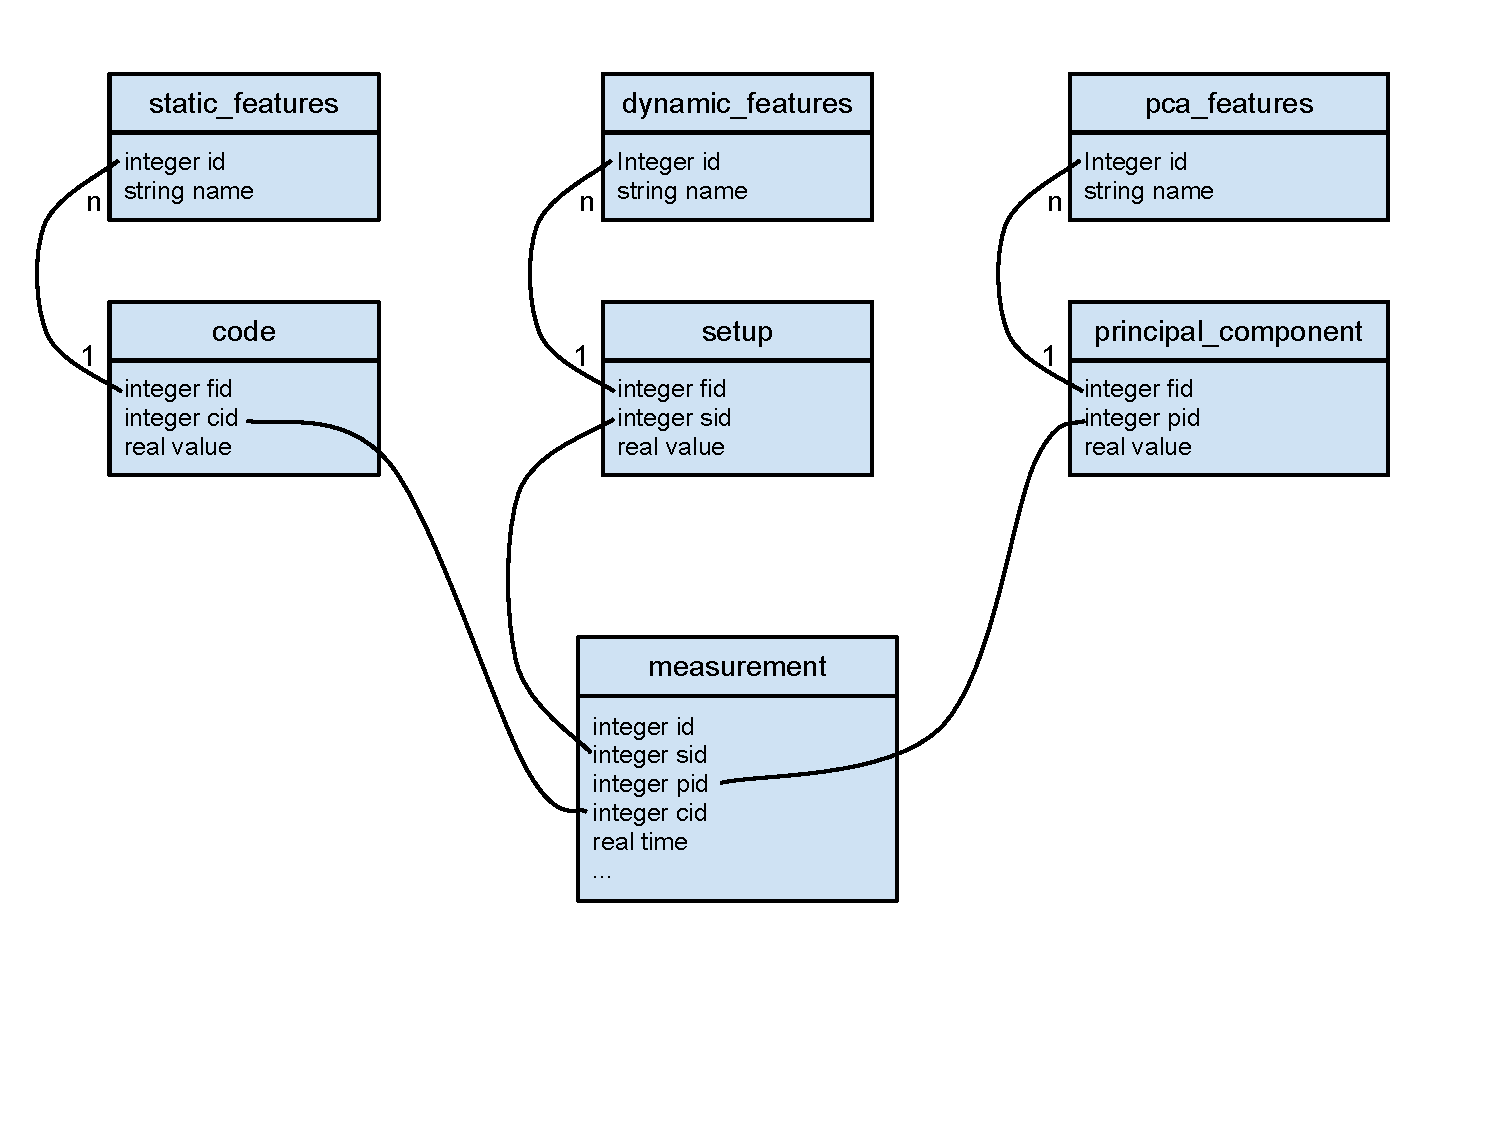
\includegraphics[width=0.95\textwidth, trim={0 4cm 0 0}]{pics/compiler/machine_learning/ml_db_schema}
	\caption{Database layout for machine learning in Insieme}
	\label{fig:Compiler.Frontend.ml.dbLayout}
\end{figure}

\subsection{The Trainer class}

The class \type{insieme::ml::Trainer} is the most important in the machine learning part since it is envolved in almost all operations. It covers many functionalities needed to train a model. The constructor takes a path to a database file and a not yet trained model as mandatory arguments. Furthermore one can customoize the way hot to map the training values to the different classes (described in Table~\ref{tab:Compiler.Frontend.ml.GenNNoutput}) and the output stream where to write the training statistics. The latter argument is only used if the makro \constant{TRAINING\_OUTPUT} in the header file \file{trainer.h} is set to true. As mentioned earlier, the features and the training target must be set, before any training can be done. After that the training can be started by calling the function \decl{virtual double insieme::ml::Trainer::train(Optimizer\& optimizer, ErrorFunction\& errFct, size\_t iterations = 0)}, passing a Shark optimizer and an error function. The optional argument \type{iterations} is only used if the model associated with the trainer uses iterative training. If so, setting it to \constant{0} will couse the trainer to use so called "early stopping" method as described in~\cite{bishop}, setting it to another value will train the model for this number of iterations.

Shark already implements a variation of this method and this variation is currently used. However, if someone wants to know how the error on the training and test dataset evolevs over the single training iterations and still use early stoping, one can exchange the call to~\decl{double insieme::ml::Trainer::earlyStopping(Optimizer\& optimizer, ErrorFunction\& errFct, Array<double>\& in, Array<double>\& target, size\_t validatonSize)} in \file{trainer.cpp} with a call to \decl{double insieme::ml::Trainer::myEarlyStopping(Optimizer\& optimizer, ErrorFunction\& errFct, Array<double>\& in, Array<double>\& target, size\_t validationSize, size\_t nBatches = 5)} and enable the training output. This function has an additional argument: the number of batches. This should be set to a value bigger than one, if the training dataset is very large. I discovered that if one has a very large training data set (several hundered thousands of patterns) convergance becomes very slow. The reason for this is that Shark does only provide batched training algorithms which update the model only once for each training iteration. Setting the number of batches to a value bigger than one will cause the trainer to subdivide the training patterns in this number of batches and do a model update after each of this batch in every iteration. Which patter is assigned to what batch is randomly (re)generated in each training iteration.

\subsection{How to add a new Model}

The interface to any model used in Insieme is defined in \file{myModel.h}. It does not only contain the definition of the abstract class \type{insieme::ml::myModel} but also the implementations of the three models currently in use. The implementations of these models does mainly forward the various calls to the Shark object, therefore the interface is very similar to the one of Shark \type{Model}. However, they are also responsible to store some data which is mainly used for reflection like for example the name of the model and some flags like if the model needs iterative training or not. Furthermore, one has to take care, that all used getters return valid numbers, which for example is not the case for the function \decl{const unsigned int Model::getOutputDimension() const} for the Shark class \type{SVM}. 

